\section{Experiment and Analysis}
\label{sec:experiment}
The following experiment will measure several architectural-independent metrics of \SA solver and evaluate the architectural characteristics. Section~\ref{sec:setup} will introduce the experiment environment first. The experiment would be classified into three categories: Section~\ref{sec:computation} analyzes the computation resource related metrics including various instruction ratio, branch misprediction rate, floating point operation ratio, etc. Section~\ref{sec:memory} presents the result of memory footprint including the memory utilization, memory-related instruction ratio and cache miss rate. Section~\ref{sec:comparison} will make comparison of the two versions of \SA solvers with respect to the decrease of accuracy and the change of performance.
\subsection{Experiment Setup}
\label{sec:setup}
The experiment is carried out by a C-language \SA solver under 32-bit GNU/Linux 2.6.43. The CPU is Intel Core i7-2600@3.40GHz with 4 cores. L1 cache includes a 4 $\times$ 32 KB instruction cache and 4 $\times$ 32 KB data cache. L2 cache is 4 $\times$ 256 KB while the shared L3 cache is 8 MB. The input data sets were generated randomly and classified into three categories according to different sizes as in Table~\ref{tab:sizes}.

\begin{table}
  \centering
  \begin{tabular}{|l|l|l|}\hline
  \textbf{Data Set} & \textbf{Text file size} & \textbf{Number of equations}\\\hline
  Small & 19KB & 128 \\\hline
  Middle&127KB&512\\\hline
  Large&148KB&1024\\\hline
  \end{tabular}
  \caption{Size of different data sets}\label{tab:sizes}
\end{table}

\subsection{Computation Resource}
\label{sec:computation}
Computation Resource includes the ratio of different kind of instructions as well as other categories of CPU-related metrics such as memory/branch instruction ratios, branch misprediction rate under different prediction strategies etc. This part of metrics are measured by the binary instrument framework Pin-Tool and the performance evaluation tools VTune Amplifier provided by Intel. The following statistics are collected by running the solver using the different data sets except where noted.
\subsubsection{Instruction Ratio}
In this part I measure the ratio of memory and branch related instructions to reveal the effect of jump/branch instructions to the overall performance. The statistics is shown in the Figure~\ref{fig:ratio}. From the graph we could observe that the memory ratio is at a high level($>=40\%$) while the branch-related instructions take about 20\% of the overall instructions. This phenomenon could be ascribed to the frequent condition judgement of temperature change. 
\begin{figure}[ht]
\centering
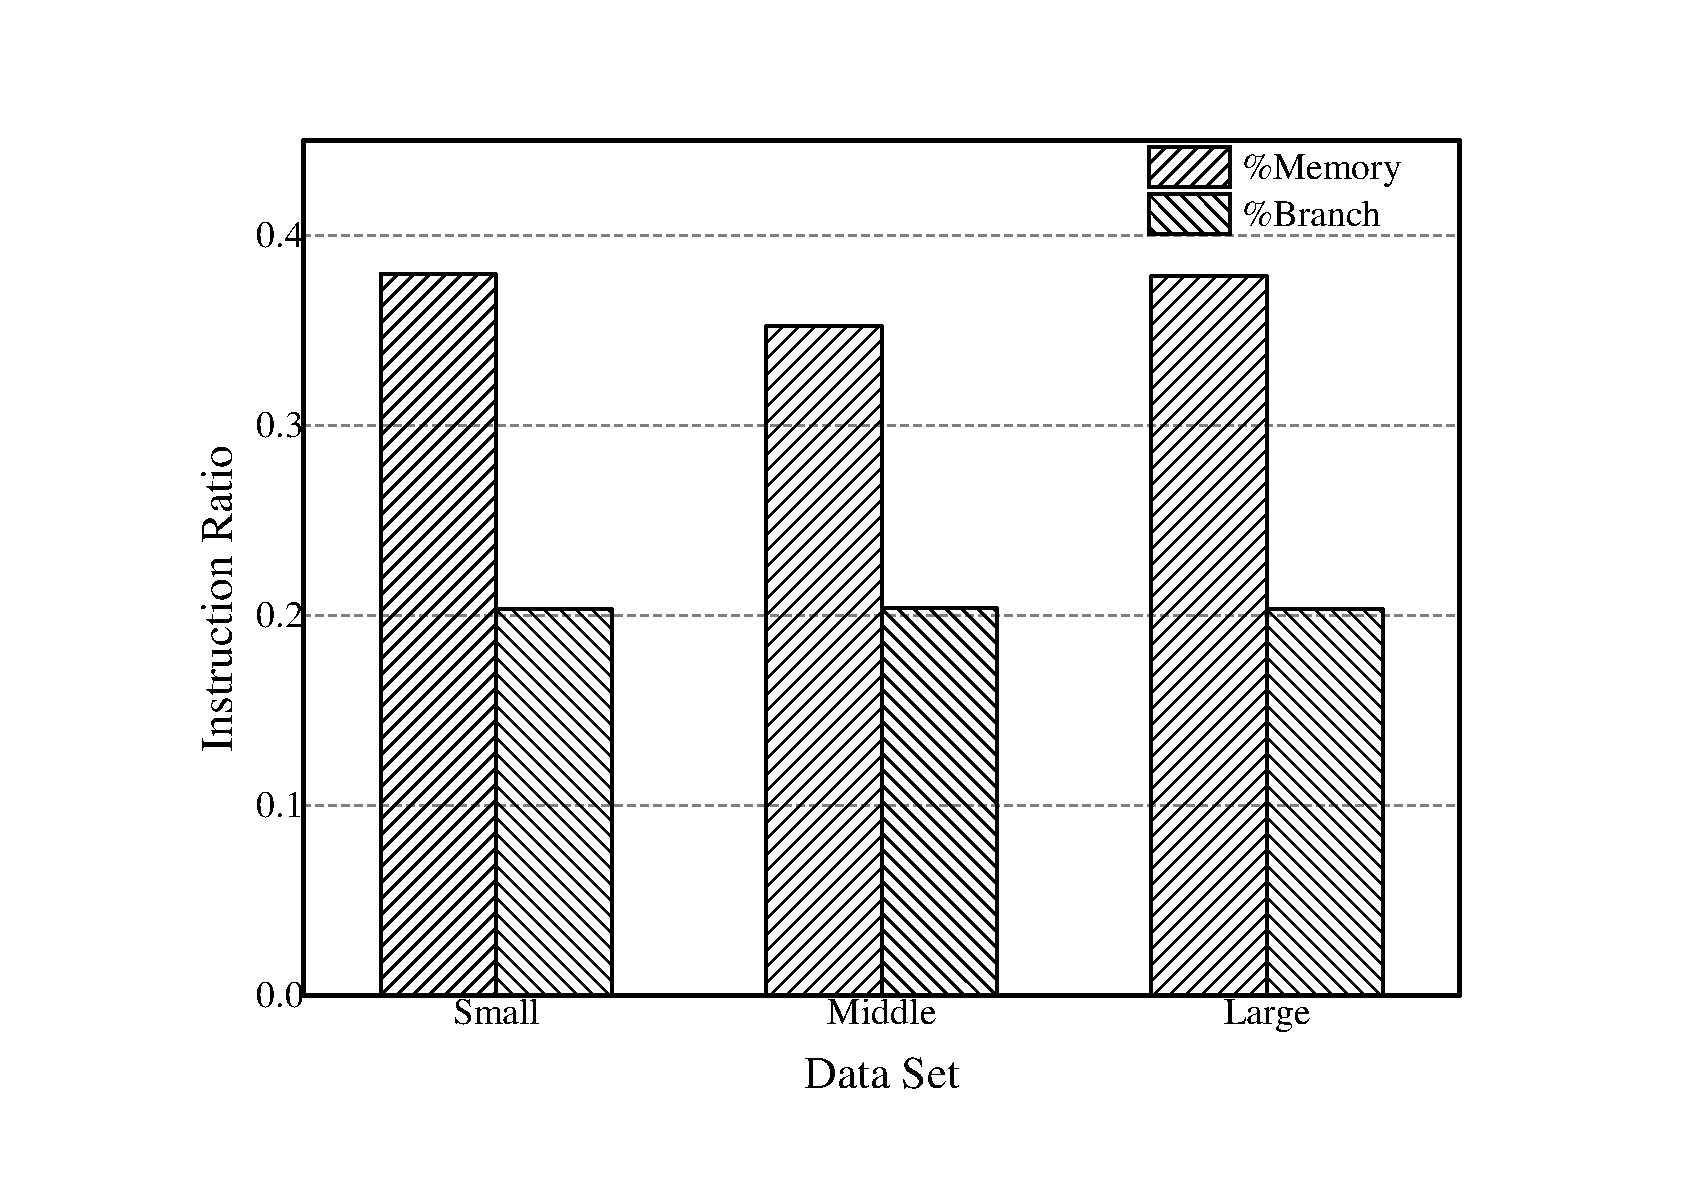
\includegraphics[width=0.50\textwidth]{graph/ins_ratio.pdf}
\caption{Instruction Ratio.}
\label{fig:ratio}
\end{figure}

\subsubsection{IPC and MPC}
\begin{figure}[ht]
\centering
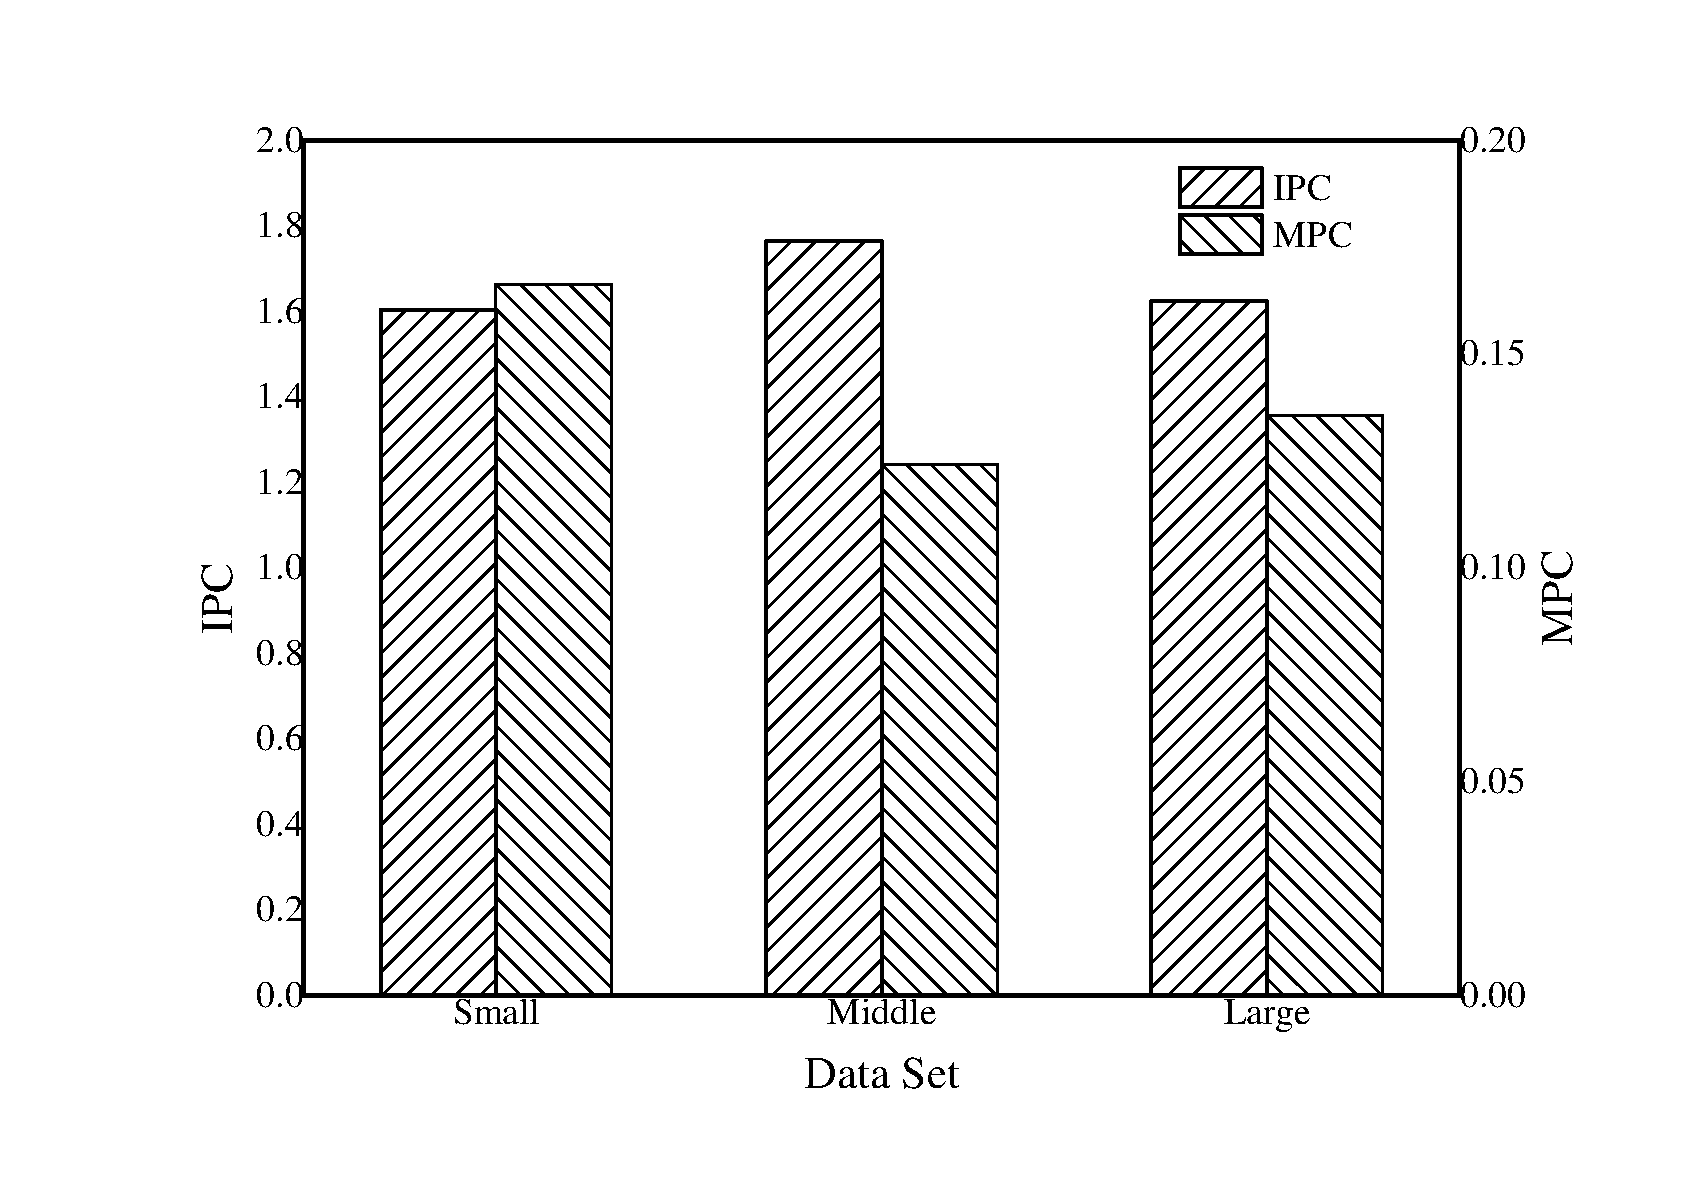
\includegraphics[width=0.50\textwidth]{graph/IPC_MPC.pdf}
\caption{Instruction per Cycle and Memory Access per 1000 Cycles.}
\label{fig:ipc_mpc}
\end{figure}

\subsubsection{Branch Misprediction Ratio }
Branch misprediction is also a significant contributor to stall cycle and slowdown of the instruction. Modern processor chips adopt different prediction strategies to prevent the miss penalty of cache miss. In this experiment we simulate three different prediction algorithms: one-bit, two-bits and two-level strategy and measure the branch misprediction rate respectively.

\begin{compactitem}
\item \textbf{One-bit strategy}: The simplest algorithm of branch prediction. A memory contains a bit indicating whether the branch is recently taken or not.
\item \textbf{Two-bits strategy}: To remedy the shortcoming of one-bit strategy, 2-bit prediction scheme adopts a finite state automata in which a prediction must miss twice before a prediction is changed.
\item \textbf{Two-level strategy}: Branch predictor that use the behavior of other branches to make a prediction called correlating predictors or two-level predictors. Existing correlating predictors add information about the behavior of the most recent branches to decide how to predict a given branch.
\end{compactitem}
Figure~\ref{fig:predict} shows the branch misprediction rate under the three strategies. From the graph we could observe that the misprediction rate is a little higher than the average computation intensive programs ($>=0.3$) at simple prediction strategy of one-bit prediction. The misprediction rate decreases notably when more complex prediction algorithm is adopted like two-level strategy. The main part of the program includes a loop of which the condition consists of a randomly generated number thus the branch behavior is much more unpredictable.

\begin{figure}[ht]
\centering
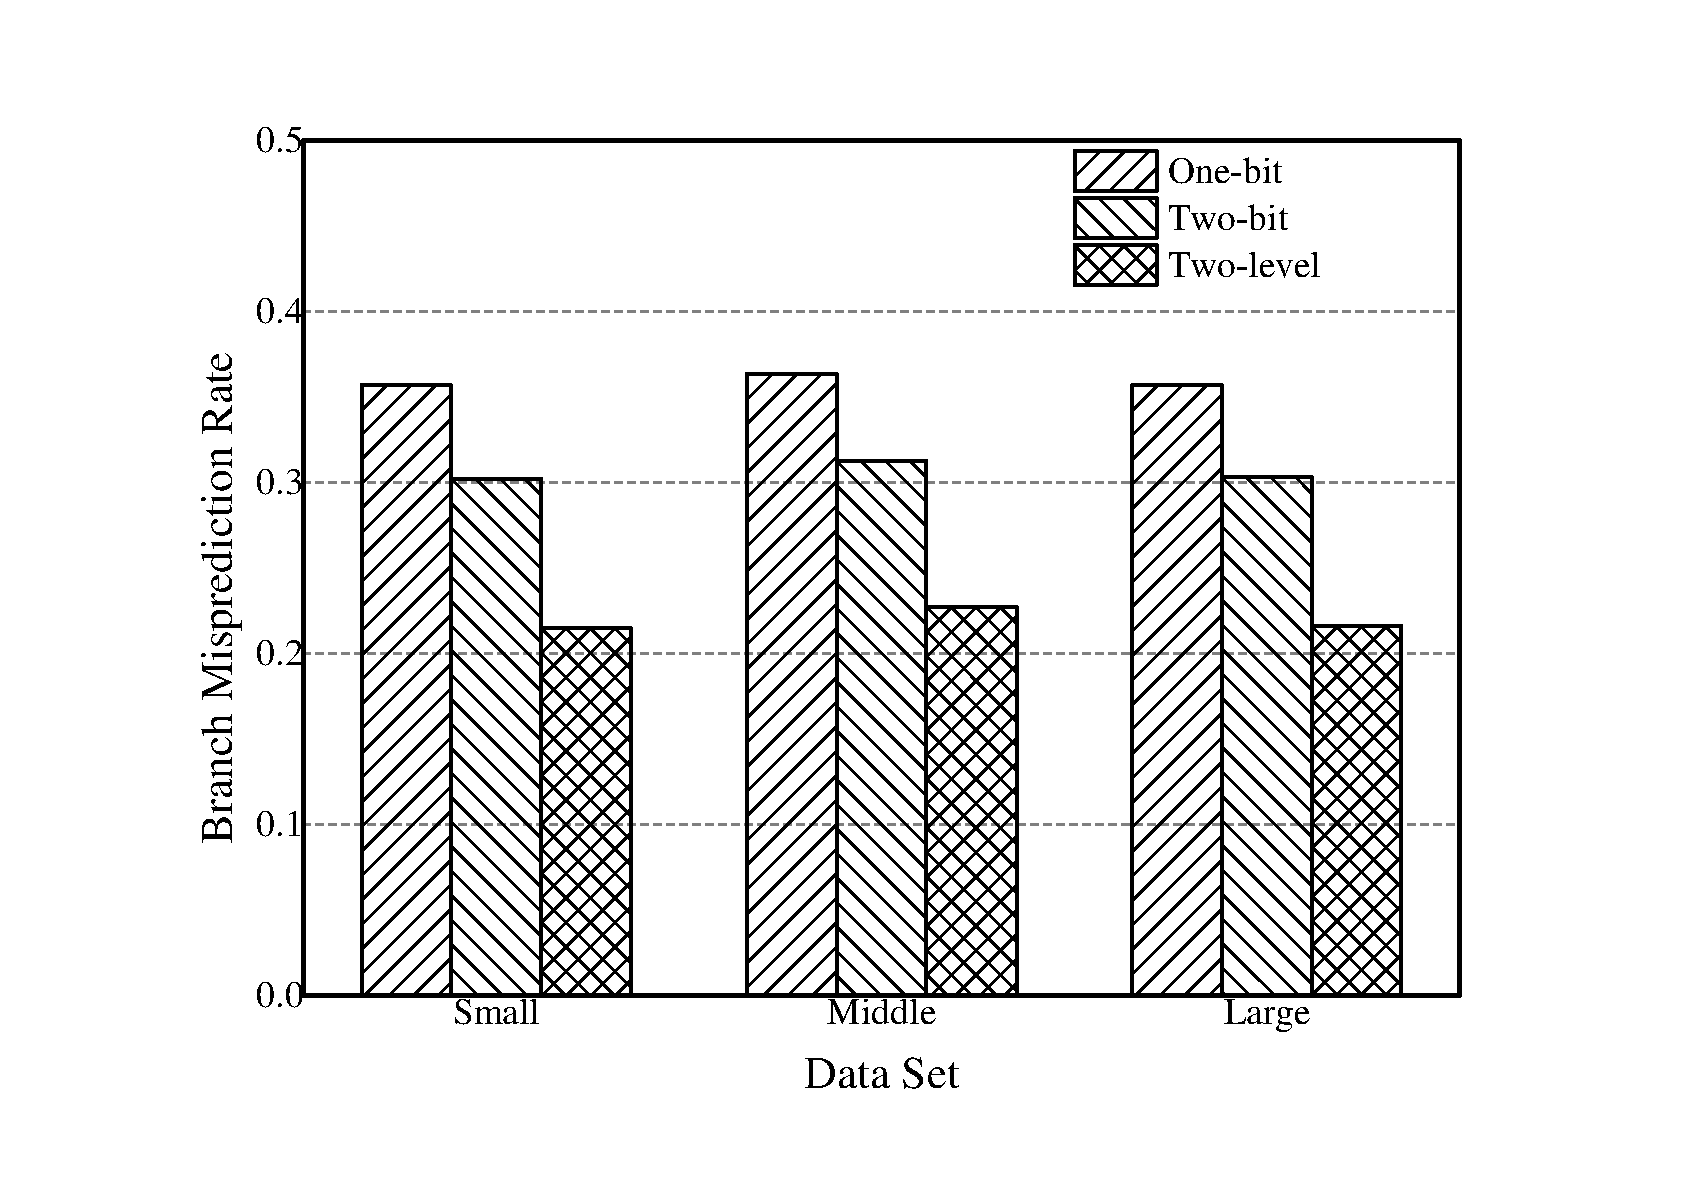
\includegraphics[width=0.50\textwidth]{graph/predict.pdf}
\caption{Branch Misprediction Rate under Different Prediction Strategies.}
\label{fig:predict}
\end{figure}

\subsection{Memory Footprint}
\label{sec:memory}

\begin{figure}[ht]
\centering
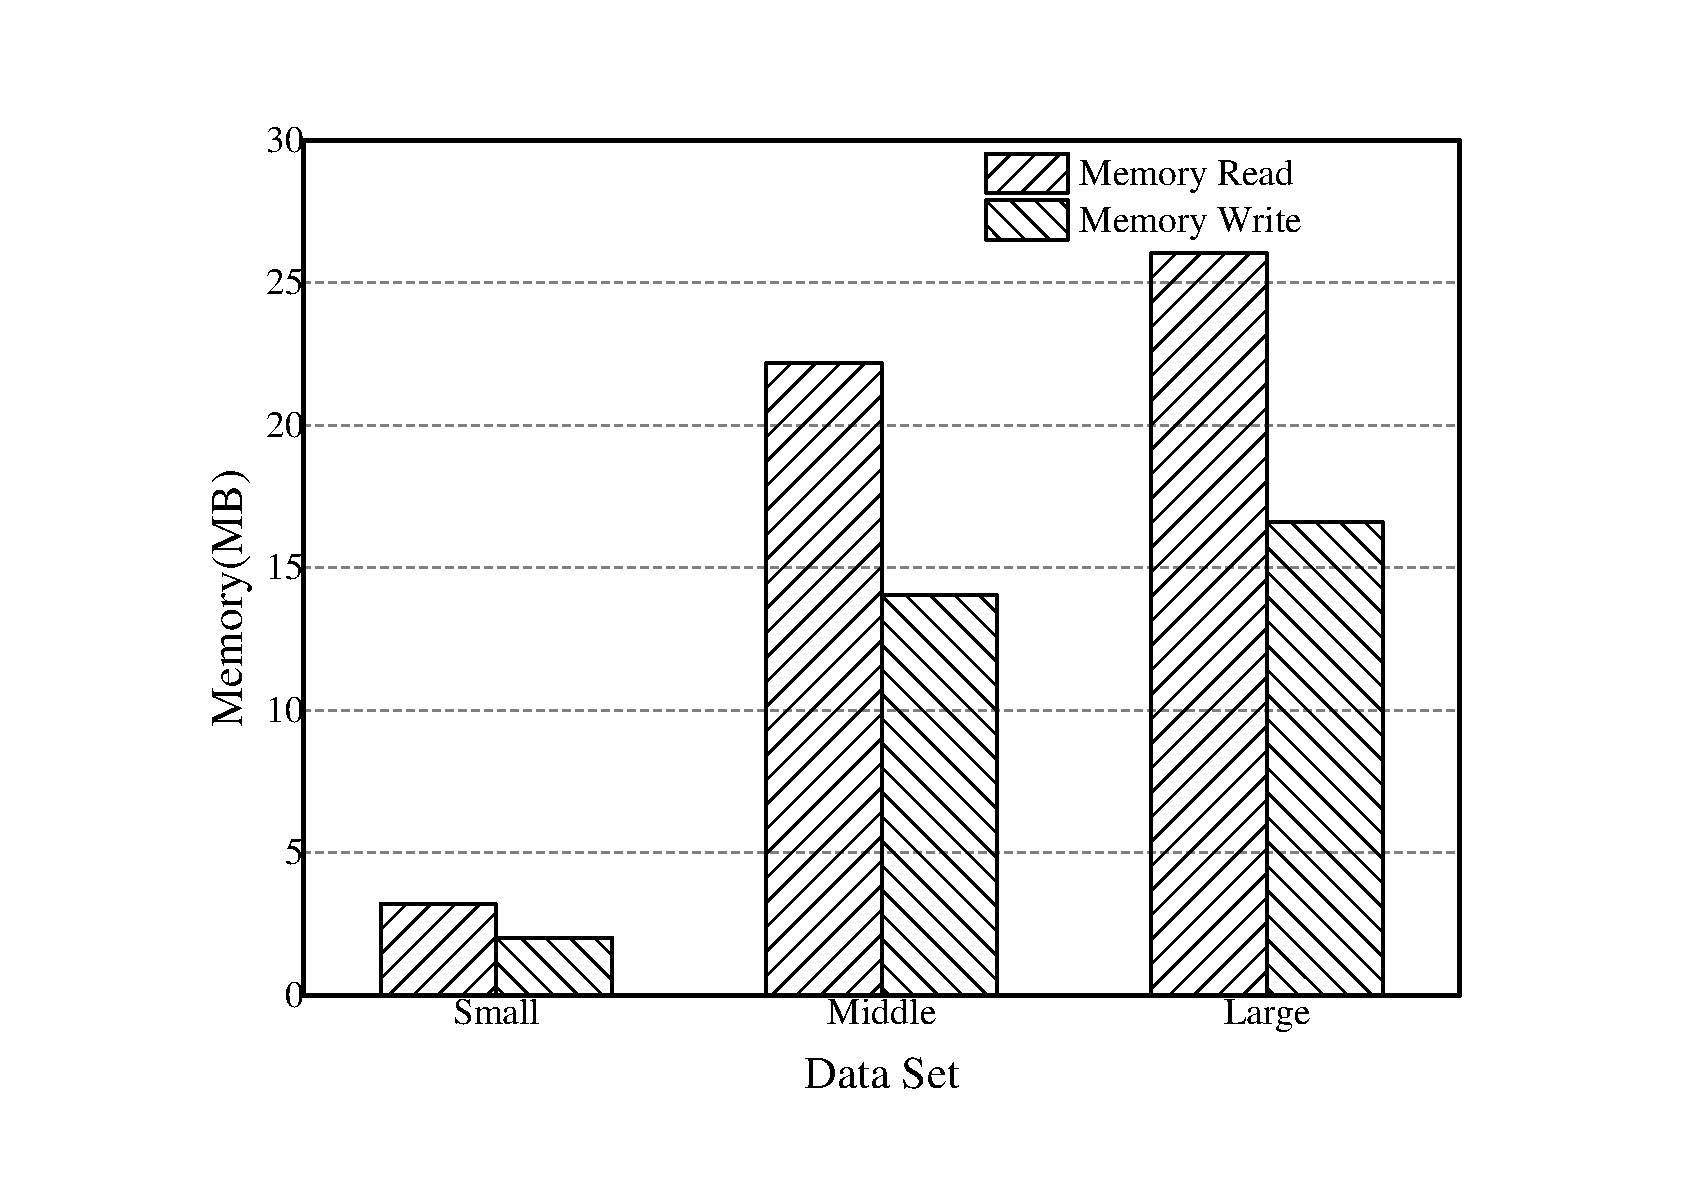
\includegraphics[width=0.50\textwidth]{graph/memory.pdf}
\caption{Memory Footprint of Read and Write.}
\label{fig:memory}
\end{figure}
\subsection{Comparison of Two Versions}
\label{sec:comparison} 